\chapter{Relevant Background}
\section{Data set}

In the context of Computer Science, very often our goal is to develop machines that can assist or automate the process of solving real-world problems. Firstly, however, we must find ways to express these problems numerically. This is were ``data sets" come in.

Although the recurrent usage of the term ``data set" in scientific work, there is not a clear definition established. It is possible, however, to observe the regular presence of four related features: grouping, content, relatedness e purpose \cite{ren2010}.
For the scope of this work, the term data set is invariably associated with the idea of a collection of samples. Each sample is a sequence of features, where the {\em i-th} feature of all instances belong to a same set of symbols $f_i$.

Succinctly, consider $S$ a sequence of samples and
$F \coloneqq  \{f_i \mid f_i \textnormal{ is a set of symbols}\}$. Then, the dataset $D$ is defined as:
$$D\coloneqq [d_{ij}] \mid d_{ij} \in f_j, \forall i \in [1, |S|], \forall j \in [1, |F|]$$

\subsubsection{Example of a canonical data set} \label{irisdataset}

The table bellow illustrates an examples of data set, where each row represents a \textbf{sample}, and each column a \textbf{feature}.

\begin{table}[H]
	\begin{tabular}{ c || *{5}{c|}}
		& \textbf{Sepal length} & \textbf{Sepal width} & \textbf{Petal length} & \textbf{Petal width} & \textbf{Species} \\
		\hline
		1 & 5.1	& 3.5 & 1.4 & 0.2 & I. setosa \\
		2 & 4.9 & 3.0 & 1.4 & 0.2 & I. setosa \\
		3 & 4.7 & 3.2 & 1.3 & 0.2 & I. setosa \\
		… & … & … & … & … & … \\
	\end{tabular}
	\caption{The first three samples of the Iris flower data set.}
\end{table}

Iris flower is an example of data set broadly used in the machine learning demonstrations, being usually interpreted as a classification problem where the feature {\em Species} will be learned from its adjacent features. In that scenario, {\em Species} is denominated \textbf{target feature}.

\subsection{Data set as a collection of vectors in the $\mathbb{R}^n$}

A data set can have each one of its nominal features enumerated. I.e., mapped to an element of $\mathbb{N}$. Such set could then be expressed as a collections of vectors in $\mathbb{R}^n$.
Consider the data set bellow:

\begin{table}[H]
	\begin{tabular}{ c | *{11}{|c}| }
		& \textbf{Age}
		& \textbf{Gen.}
		& \textbf{TB}
		& \textbf{DB}
		& \textbf{Alk.}
		& \textbf{Sgpt}
		& \textbf{Sgot}
		& \textbf{TP}
		& \textbf{ALB}
		& \textbf{A/G}
		& \textbf{S} \\
		\hline
		1 & 65 & Female & 0.7 & 0.1 & 187 & 16 & 18 & 6.8 & 3.3 & 0.9 & 1 \\
		2 & 62 & Male & 10.9 & 5.5 & 699 & 64 & 100 & 7.5 & 3.2 & 0.74 & 1 \\
		3 & 62 & Male & 7.3 & 4.1 & 490 & 60 & 68 & 7 & 3.3 & 0.89 & 1\\
		… & … & … & … & … & … & … & … & … & … & … & … \\
	\end{tabular}

	\caption{The first three samples of the Indian Liver Patient Dataset (ILPD)}
\end{table}

Composed by 583 samples and 11 features, the data set ILPD has a nominal feature $Gender \coloneqq \{Male, Female\}$. {\em Gender} can, of course, be mapped on $\{0, 1\}$. ILPD can finally be expressed by the figure bellow:

\begin{figure}[H]
	\centering
	\captionsetup{justification=centering}

	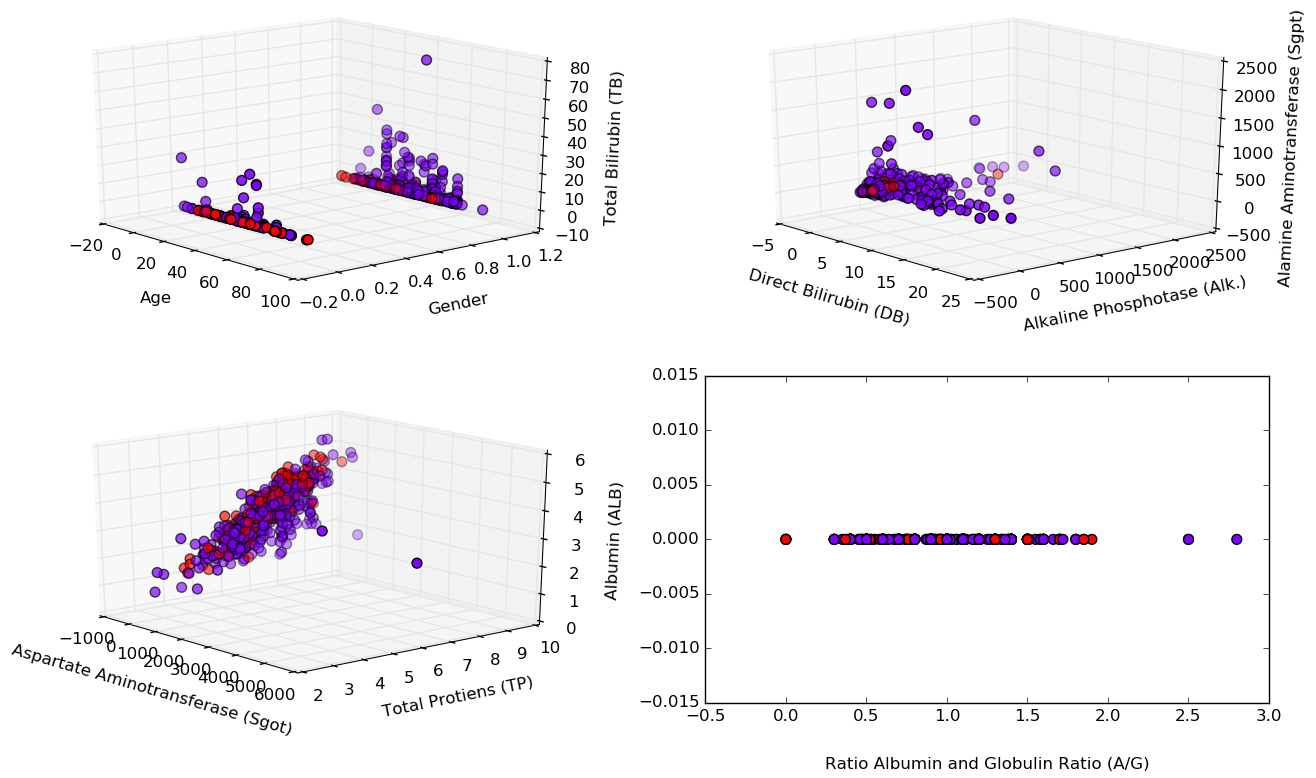
\includegraphics[scale=.4]{experiments/displaying_ilpd}
	\caption{The data set ILPD's samples mapped onto the $\mathbb{R}^n$, where each of its features is an axis in one graph, except for $S \coloneqq \{1, 2\}$, which was represented by the vertices' colors.}
	\label{fig:disp_ilpd}
\end{figure}

Considering the many graphs required to display the data set, it is quite difficult to identify a plausible distribution for ILPD. We define here our first encouragement towards the study of dimensionality reduction: the identification of the most significant features (i.e., that maximize variance) and plotting of those might result on simpler and more intuitive representations. Furthermore, it would also be interesting to combine the existing features to create new ones that are even more representative.

\subsection{Modern Problems and Applications}

Differently from Iris flower or ILPD data set, data sets associated with modern problems are often very dense, i.e., data sets containing many samples and/or features. Although the high number of samples is essentially benefic, a high number of features might be irrelevant or even unconstructive to the learning process \cite{cay2005}.

\begin{table}[H]
	\begin{tabular}{ c | *{4}{|c}| }
		& A & B & … & AAAV \\ \hline
		1 & 0.0111486888670454 & -0.01541263850539861 & … & 0.007440367302352156 \\
		2 & 0.03016080450207878 & 0.1772161342899135 & … & 0.01309011094914101 \\
		… & … & … & … & … \\
		8200 & 0.02680808496910305 & -0.0320375843317954 & … & 0.1772161342899135 \\
	\end{tabular}

	\caption{A data set with 8200 samples and 100 features.}
\end{table}

In many cases, there are indicatives that the data set lie near a lower-dimensional manifold embedded in the $\mathbb{R}^n$ \cite{gho2006}. For the data set above, in special, the $\mathbb{R}^{100}$. A second encouragement can then be set: it is possible that the data set might be shrunk by combining similar (linearly dependent) features or eliminating the ones that poorly contribute towards the learning process. In order to do this, one must be able to qualify the “contribution” of each feature or even identify dependencies between features.

\section{Probability Theory}
\subsection{Feature Standardization}
Many of the methods ahead will require the data set to be centered in the origin. To center a data set $X$, we build a data set $X'$ s.t. each column has zero mean and it is contracted by its standard deviation:
$$X'_{.j} = \frac{X_{.j} - \mu}{\sigma} \textnormal{, where}$$
\begin{enumerate}
	\item $X_{.j}$ is the j-th column of the matrix $X$.
	\item $\mu$ is the mean of $X_{.j}$.
	\item $\sigma$ is the standard deviation of $X_{.j}$.
\end{enumerate}

\subsection{Centering Matrix}
The symmetric matrix $H$ is named the \textbf{centering matrix} when the multiplication of it by a vector $X$ produces the same effect of subtracting the mean of the components from each component of $X$. $H$ is defined as:
$$
H = I_n - \frac{1}{n}\textbf{11}^T \textnormal{, where:}
$$
\begin{enumerate}
	\item $I_n$ is the identity matrix of order $n$.
	\item $\textbf{1}$ is the column vector of 1's.
\end{enumerate}

\subsection{Variance}
Variance is the measure which describes how far the samples in a given set X vary. For the scope of this project, only discrete probabilities will be considered. That is, if $X$ represents a variate with known distribution $P(x)$, where $P(x) = k \in \mathbb{R}^{+}, \forall x \in X$ and $\sum_{x \in X} P(x) = 1$, and $\mu$ is the population mean of $X$, then \cite{ross2010introductory}:
\begin{align*}
	Var(X) = \frac{1}{n} (X-\mu) \cdot (X-\mu) = \frac{1}{n} \sum_{x \in X} (x - \mu)^2
\end{align*}

\begin{remark}
	If $var(X) = 0$, then it can be easily asserted that all variables in $X$ assume the exact same value by using the elementary properties of the inner product.
\end{remark}

\begin{example}
	If $X=\{1, 2, -2, 4\}$ and $\mu = \frac{1}{4} \sum X_i = \frac{1+2-2+4}{4} = 1.25$, then
	\begin{align*}
	var(X) &= \frac{1}{4} \sum (X_i - \mu)^2 \\
	&= \frac{(1-1.25)^2 + (2-1.25)^2 + (-2-1.25)^2 + (4-1.25)^2}{4} \\
	&= 4.6875
	\end{align*}
\end{example}

\begin{example}
	The variance of the Sepal length feature in the Iris flower data set can be calculated as:
	\begin{align*}
	var(X) &= \frac{1}{150} \sum (X_i - \mu)^2 \\
	&= \frac{1}{150} [(5.1-5.84)^2 + (4.9-5.84)^2 + \cdots + (5.9-5.84)^2] \\
	&= \frac{102.17}{150} = .681122
	\end{align*}
\end{example}

\subsection{Covariance}

The covariance measures the variance of two random variates in respect to each other. Formally, if $X$ and $Y$ are two given random variates with known mean population distribution $\mu_X$ and $\mu_Y$, respectively, then
$$\sigma(X, Y) = \frac{1}{n} (X - \mu_X) \cdot (Y - \mu_Y) $$

Simply putting, the covariance of two random variables $X$ and $Y$ can be interpreted as one of the following behaviors:
$$
\sigma(X,Y) = \begin{cases}
\sigma_{xy} > 0 \implies \textnormal{X tends to increase as Y increases.}\\
\sigma_{xy} < 0 \implies \textnormal{X tends to increase as Y decreases.}\\
\sigma_{xy} = 0 \implies \textnormal{X and Y are completely unrelated.}
\end{cases}
$$

\begin{remark}
	For a random variate $X$, $var(X) = \sigma(X, X)$.
\end{remark}

\paragraph{Covariance Matrix of Features in a Centered Data Set}

Let $D$ be a data set, $H$ the centering matrix and $HD_{\_i}$ the {\em i-th} feature column of the centered data set $HD$, the covariance between each one of its features can be represented by the matrix:
\begin{align*}
\Sigma &= [\sigma_{xy}]_{n \times n} \\
&= \begin{bmatrix}
\sigma(HD_{\_0}, HD_{\_0}) & \sigma(HD_{\_0}, HD_{\_1}) & \cdots & \sigma(HD_{\_0}, HD_{\_n-1}) \\
\sigma(HD_{\_1}, HD_{\_0}) & \sigma(HD_{\_1}, HD_{\_1}) & & \sigma(HD_{\_1}, HD_{\_n-1}) \\
\vdots &&& \vdots \\
\sigma(HD_{\_n-1}, HD_{\_0}) & \sigma(HD_{\_n-1}, HD_{\_1}) & \cdots & \sigma(HD_{\_n-1}, D_{\_n-1})
\end{bmatrix} \\
&= \frac{1}{n} (HD)^T HD \\
&= \frac{1}{n} D^T H^T H D \\
 &= \frac{1}{n} D^T H D
\end{align*}

Where $H$ is the \textbf{centering matrix}.

\subsection{Correlation}

The correlation is a measure of the direction and strength of a linear relationship among variables. Let $X$ and $Y$ be two random variables, $r(X, Y)$, i.e., the correlation between $X$ and $Y$ is defined as \cite{ross2010introductory}:
\begin{align*}
	r(X, Y) = \frac{\sigma(X, Y)}{\sigma_X \sigma_Y},
\end{align*}

where $\sigma_X$ and $\sigma_Y$ are the standard deviations of the variables $X$ and $Y$, respectively. Of course, $r(X, Y) \in [-1, 1]$.

\begin{remark}
	If $X$ and $Y$ are two random variables and $\sigma(X, Y) = 1$, $X=Y$.
\end{remark}

\subsubsection{Correlation Matrix of Features in a Centered Data Set}

Let $D$ be a data set, $H$ the centering matrix and $HD_{\_i}$ the {\em i-th} feature column of the centered data set $HD$. The correlation between each one of its features can be represented by the matrix:
\begin{align*}
	corr(D) &= \begin{bmatrix}
		1 & \frac{\sigma(HD_{\_0}, HD_{\_1})}{\sigma_{HD_{\_0}} \sigma_{HD_{\_1}}} & \cdots & \frac{\sigma(HD_{\_0}, HD_{\_n-1})}{\sigma_{HD_{\_0}} \sigma_{HD_{\_n-1}}} \\
		\frac{\sigma(HD_{\_1}, HD_{\_0})}{\sigma_{HD_{\_1}} \sigma_{HD_{\_0}}} & 1 & \cdots & \frac{\sigma(HD_{\_1}, HD_{\_n-1})}{\sigma_{HD_{\_1}} \sigma_{HD_{\_n-1}}} \\
		\vdots & \vdots && \vdots \\
		\frac{\sigma(HD_{\_n-1}, HD_{\_0})}{\sigma_{HD_{\_n-1}} \sigma_{HD_{\_0}}} & \frac{\sigma(HD_{\_n-1}, HD_{\_1})}{\sigma_{HD_{\_n-1}} \sigma_{HD_{\_1}}} & \cdots & 1
	\end{bmatrix}
\end{align*}

\section{Numerical Analysis}
\subsection{Eigenvalues and Eigenvectors of a Matrix}

Given a matrix $A \ne 0 \in \mathbb{R}^{2n}$, a vector $v \in \mathbb{R}^n$ is said to be an \textbf{eigenvector} of $A$ if the multiplication $Av$ does not change the direction of $v$; that is:
$$\exists \lambda \in \mathbb{R} \mid Av = \lambda v \textnormal{, where}$$
$\lambda$ is the \textbf{eigenvalue} associated to the eigenvector $v$.

\subsection{Spectral Decomposition of a Matrix}

If $[M]_{n\times n}$ is a symmetric matrix of rank $n$ and admits $n$ pairs of eigenvalues $\lambda$ and eigenvectors $[V]_{n\times n} = [v_0, v_1, v_2, ..., v_{n-1}]$, such that $V$ is an orthogonal matrix (i.e., $V^TV=I_n$), then
$$MV = V \lambda$$

$\lambda = diag(\sigma_0, \sigma_1, ..., \sigma_{n-1})$ is the diagonal matrix, where $\sigma_i$ is the eigenvalue associated to the eigenvector $v_i$ \cite{cox2001}. Furthermore, $V$'s columns are linear independent, hence $V$ is invertible.
\begin{align*}
	MV &= V \lambda \\
	MVV^T &= V \lambda V^T \\
	M &= V \lambda V^T
\end{align*}

\subsection{Singular Value Decomposition}
\label{sec:svd}
If $M \in \mathbb{R}^{m \times n}$, then $\exists U \in \mathbb{R}^{m \times m}, V \in \mathbb{R}^{n \times n}$ and $\Sigma =  diag(\sigma_0, \dots, \sigma_{n-1})$ conditioned to $\sigma_i \ge \sigma_{i+1} \ge 0, \forall \sigma \in [0, n)$ s.t. \cite{gan2008}
$$M = U\Sigma V^T$$

\begin{theorem}
	\label{th:svd-aat}
	If $A = U \Sigma V^T$, $AA^T = U \Sigma^2 U$ and $A^TA = V \Sigma^2 V$.
\end{theorem}
\textbf{Proof}
\begin{align*}
	A^TA &= (U\Sigma V^T)^T(U\Sigma V^T) \\
	&= V \Sigma^T U^T U \Sigma V^T \\
	&= V \Sigma \Sigma V^T \\
	&= V \Sigma^2 V^T
\end{align*}

Proving $AA^T = U \Sigma^2 U^T$ is analogous to the above.

\section{Topology}
\subsection{Manifolds}

Intuitively, $n$-dimensional topological manifolds are sets that are ``locally Euclidean" \cite{lee2009}. In other words, they can be decomposed into sub sets that can be mapped to the $\mathbb{R}^n$.

Formally, a set $M$ is said to be a \textbf{$n$-dimensional topological manifold} $\iff M$ is a paracompact Hausdorff topological space $\mid \forall p \in M, p \in U_p$, where $U_p$ is an open set that is homeomorphic to an open set $V_p$ of the Euclidean space $\mathbb{R}^n$ \cite{lee2009}.

From now on in this report, we will use the word manifold to refer to a $n$-dimensional topological manifold.

\subsubsection{Charts}
The pair $(U_i, \phi_i)$ is called a \textbf{coordinate chart} or \textbf{chart} on $M$ if $U \in M$ and $\phi_i$ is a \textbf{homeomorphism} such that $\phi_i(U_i) = V_i \subseteq \mathbb{R}^n$ \cite{lee2002}.

\subsubsection{Atlas}

A set $A = \{(U_i, \phi_i)\}_{i \in A}$ is said to be an \textbf{atlas} on a manifold $M$ if $\cup_{i \in A} U_i = M$ \cite{lee2002}.

\begin{example}
	The $\mathbb{R}^n$ is, directly, a manifold.
\end{example}

\begin{example}
	A n-dimensional sphere is a manifold. Earth, in special, is a 3-dimensional sphere and its stereographic projection is its mapping to the $\mathbb{R}^2$ \cite{stereo_proj}.

	\begin{figure}[H]
		\centering
		\captionsetup{justification=centering}

		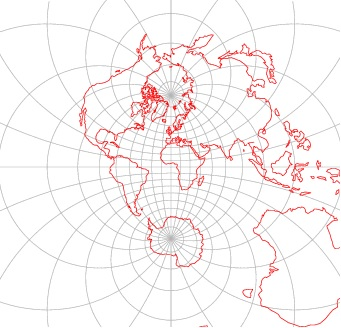
\includegraphics[scale=.8]{stereo_earth}
		\caption{Stereographic projection applied to Earth.}
		\label{fig:stereographic_earth}
	\end{figure}
\end{example}

\section{Graph Theory}
\subsection{Graphs}

Let $G$ be the pair $(X, U)$. $G$ is defined as a \textbf{graph} \cite{berge1973}, where
\begin{enumerate}
	\item $X$ is a set of objects called \textbf{vertices}.
	\item $U$ is a family of elements $u_i \in X\times X$ called arcs.
\end{enumerate}

\subsubsection{Basic Concepts \cite{berge1973}}
\begin{description}
	\item[Multiplicity] If $G=(X, U)$ and $(x, y) \in X\times X$, the multiplicity $m_g^+(x, y)$ of $x, y$ is defined to be the number of arcs with initial endpoint $x$ and terminal endpoint $y$. Furthermore:
	\begin{enumerate}
		\item $m_G^-(x, y) = m_G^+(y, x)$
		\item $m_G(x, y) = m_G^+(x, y) + m_G^-(x, y)$
	\end{enumerate}

	\item[Degree] If $G=(X, U)$ is a graph and $x\in X$, the degree $d(x)$ of $x$ is defined \cite{may1972} as
	$d(x) = 2n_s  + n_n$, where $n_s$ is the number of arcs self-incident at $x$ (i.e., $\{(x, x)\}$) and $n_n$ is the number of arcs incident at $x$.

	\item[Adjacency Matrix] If $G=(X, U), X=\{x_1, x_2, \dots, x_n \}$, define the adjacency matrix $A=[a_{ij}]_{n\times n}$ associated with graph $G$, where $a_{ij} = m_G^+(x_i, x_j)$.
\end{description}

\subsubsection{Further Specifications}

\begin{description}
	\item[Undirected graph] ``All graphs are directed, but sometimes the direction need not be specified" \cite{berge1973}.

	Let $G=(X, U)$ be a graph and $u_k \in U \mid u_k=(a, b)$. The element $e_i=[a, b]$ can be defined as the \textbf{edge} that links $a$ to $b$ without specifying direction. Finally, define the \textbf{undirected graph} $H$ as $(X, E)$, where $E=\{e_i\}$ is the set of edges created from $U$.

	Figure \ref{fig:graph} shows the graph \textbf{Les Miserables}, where each node is a character and each arc links two characters that have shared stage at some point during the play.

	\begin{figure}[H]
		\centering
		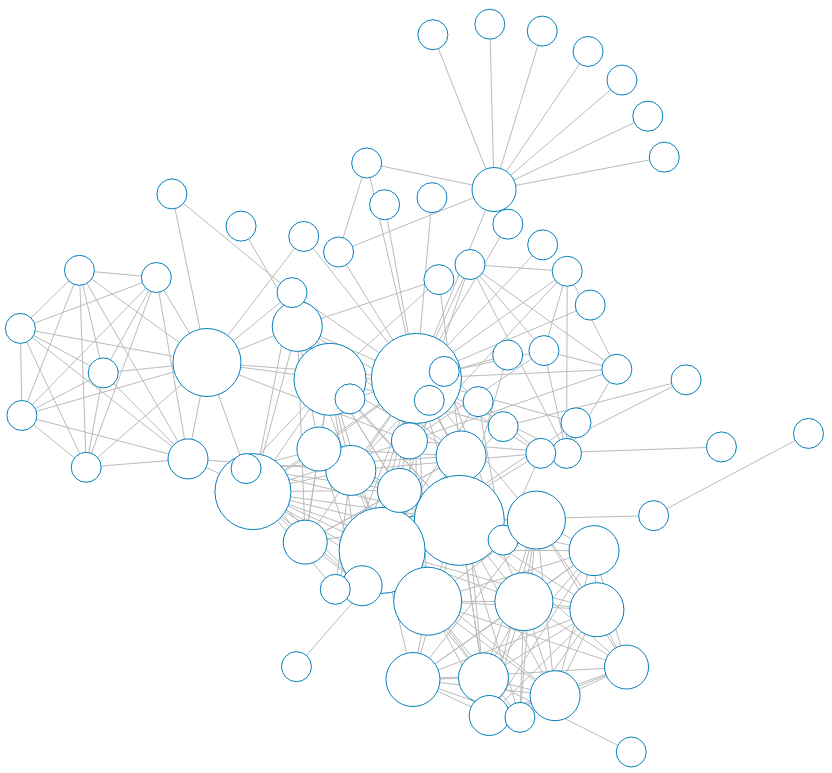
\includegraphics[width=.5\linewidth]{graphs/graph}
		\caption{The \textbf{Les Miserables} graph.}
		\label{fig:graph}
	\end{figure}

	\item[Complete graph] A graph $G=(X, U)$ is said to be complete if
	$$\forall (x, y)\in X, x\ne y, m_G(x, y) \ge 1$$

	\begin{remark}
		Let $G=(X, U), G_1=(X, E)$ and $n=|X|$. $G$ is called the complete graph $K_n$ if
		$$\forall (x, y)\in X, \exists e \in E \mid e=[x, y]$$
	\end{remark}

	\item[Weighted graph] Let $G=(X, U)$ be a graph and $w\colon U \to \mathbb{R} \mid w(u) = w_u$ be the weighted associated with arc $u$. $G$ is said to be a weighted graph.

	\item[Euclidean graph] If $G=(X, U)$ and $W=\{w_u, \forall u\in U\}\subset \mathbb{R}$, $G$ is said to be an euclidean graph if $w_u$ corresponds to the euclidean distance between the vertices connected by $u$ in a specified embedding.

	\item[Tree] Let $G$ be the graph $(V, E)$ such that $G$ is connected and admits no cycles. $G$ is  said to be a \textbf{tree} \cite{berge1973}. 

	\begin{figure}[H]
		\centering
		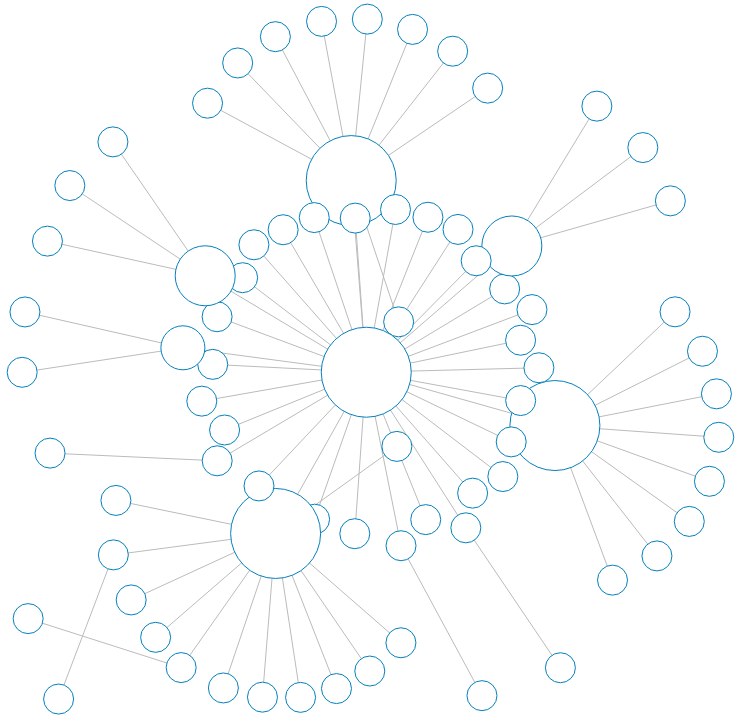
\includegraphics[width=.4\linewidth]{graphs/tree}
		\captionsetup{justification=centering}
		\caption{A tree extracted (a subgraph) from the \textbf{Les Miserables} graph.}
		\label{tree}
	\end{figure}
\end{description}

\subsection{Related Problems}

\subsubsection{Nearest-Neighbor Search}

Let $G = (X, U)$ be a weighted graph, where $ \forall u \in U, \exists w_u \in \mathbb{R}$, i.e., the weight or \textbf{length} of the arc $u$, and $n\colon U \to \{0, 1\}$ a definition of \textbf{nearness} in $G$. The nearest-neighbor search is a optimization problem that consists of finding a subgraph $H = (X, F \subseteq U) \mid f \in F \iff n(f) = 1$.

\paragraph{A Generic Algorithm for NN Search}
\begin{enumerate}
	\item $F_x \coloneqq \emptyset, \forall x \in X$
	\item $F_x \coloneqq F_x \bigcup_{\forall p \in U_x} \begin{cases}
	\{p\}, \text{if } n(p) = 1 \\
	\emptyset, \text{if } n(p) = 0 \\
	\end{cases}$
	\item $H \coloneqq (X, F), F = \cup_{x\in X} F_x$
\end{enumerate}

Let's consider two (between many)  specifications of this algorithm:

\begin{description}
	\item[K-Nearest Neighbor Search (K-NN)] Fixed $k \in \mathbb{N}$ and $U_x \subseteq U$, where $U_x$ is the set of all arcs with $x$ as initial endpoint, define:

	\begin{align*}
	n(u_x) &\coloneqq \begin{cases}
		1, \text{if }  w_{u_x} \le w_p, \forall p \in U_x - F_x \text{ and } |F_x| \le k \\
		0, \text{otherwise.} \\
		\end{cases}
	\end{align*}

	\item[$\epsilon$-Nearest Neighbor ($\epsilon$-NN)] Fixed $\epsilon \in\mathbb{R}$, define:
	\begin{align*}
		n(f) &\coloneqq \begin{cases}
			1, \text{if } w_f \le \epsilon \\
			0, \text{otherwise} \\
		\end{cases}
	\end{align*}
\end{description}

\begin{example}
	If $k=1$ and $\epsilon=60$, the graph $G$, the sub-graph $H$ found from K-Nearest neighbor algorithm and the sub-graph $I$ found from the $\epsilon$-Nearest neighbor are defined as follows:
	\begin{figure}[H]
		\begin{subfigure}{.33\linewidth}
			\centering
			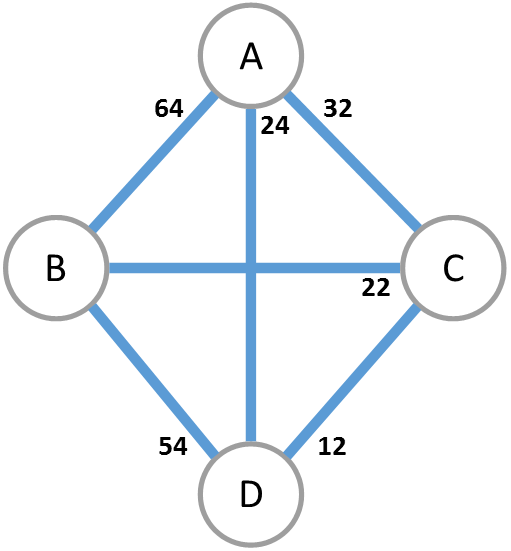
\includegraphics[width=.8\linewidth]{graphs/example-graph}
			\caption{$G$}
			\label{fig:example-graph}
		\end{subfigure}%
		\begin{subfigure}{.33\linewidth}
			\centering
			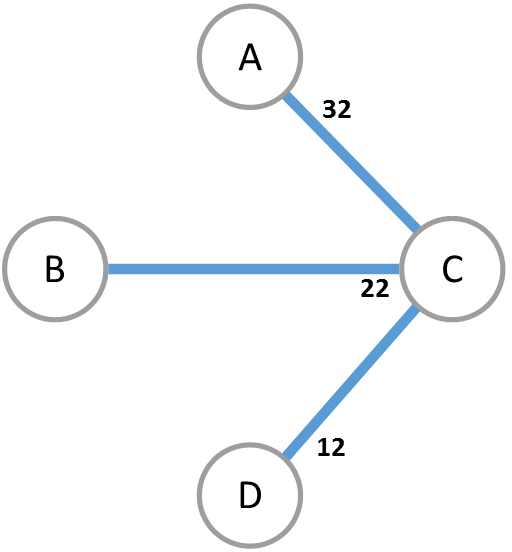
\includegraphics[width=.8\linewidth]{graphs/example-graph-nn}
			\caption{$H$}
			\label{fig:example-graph-nn}
		\end{subfigure}%
		\begin{subfigure}{.33\linewidth}
			\centering
			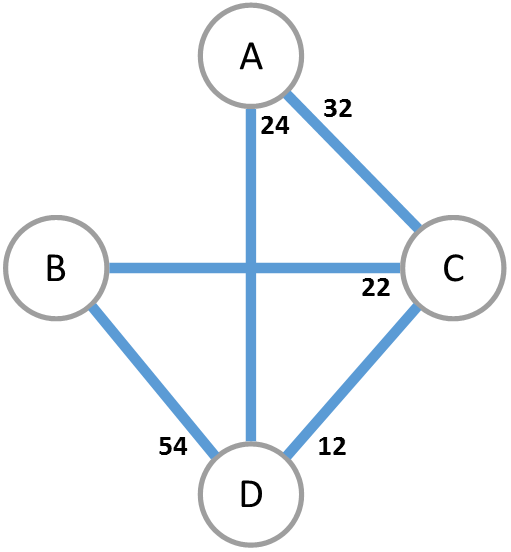
\includegraphics[width=.8\linewidth]{graphs/example-graph-en}
			\caption{$I$}
			\label{fig:example-graph-en}
		\end{subfigure}
	\end{figure}
\end{example}

\subsubsection{Single-pair Shortest-path Problem \cite{cor2011}}

Let $G=(X, U)$ be a weighted graph, a path $p(x, y)=(u_0, u_1, u_2, \dots, u_{p-2}, u_{p-1}, u_{p}) \mid u_0 = (x, \_), u_p = (\_, y), u_i \in U, \forall i \in [0, p]$, and the weight of $p$ be given by $w(p) = \sum_i^p w(u_i)$. The shortest-path weight between two vertices $x$ and $y$ is defined as:
\begin{align*}
	\sigma(x, y) = \begin{cases}
		\min \{w(p(x, y))\}, \text{ if $p(x, y)$ exists}, \\
		\infty, \text{ otherwise.}
	\end{cases}
\end{align*}

while $p(x, y)$ is the \textbf{shortest path} from $x$ to $y$.

The shortest-path between a vertex $x_0 \in X$ and all other vertices can be expressed by the tree $S=(X, F), F \subseteq U$ named \textbf{shortest-path tree}.

\paragraph{Dijkstra's Algorithm \cite{cor2011}}

Let $G=(V, E)$ be a directed weighted graph and $v_0 \in V$ the initial vertex, the shortest-path from $v_0$ to all other vertices can be found through Dijkstra's algorithm:

\begin{lstlisting}[mathescape]
    $Dijkstra(V, E, w)$:
        for $v \in $ V
            $predecessor(v_i) \leftarrow None$
            $d(v_i) \leftarrow \infty$
        $d(v_0) \leftarrow 0$
        S $\leftarrow \emptyset$
        Q $\leftarrow $ priority_queue(V, d)
        while Q $\ne \emptyset$
            u $\leftarrow$ pop_min(Q)
            for each $v \in V \mid (u, v) \in E$
                if $d(v) > d(u) + w(u, v)$
                    $d(v) \leftarrow d(u) + w(u, v)$
                    $predecessor(v) = u$
\end{lstlisting}

\begin{remark}
	Dijkstra's algorithm is based on two strategies: greedy, when extracting the vertex $u$ such that $d(u)$ is minimum, and dynamic programming, during edge relaxation (comparison and update of the $d(v)$ and $predecessor(v)$ values).
\end{remark}

\begin{example}
	Let G be the weighted graph as defined in figure \ref{fig:spa-graph}. The shortest-path between $A$ and all other vertices is described by the tree $S$ illustrated in figure \ref{fig:spa-tree}.

	\begin{figure}[H]
		\centering
		\begin{subfigure}{.4\linewidth}
			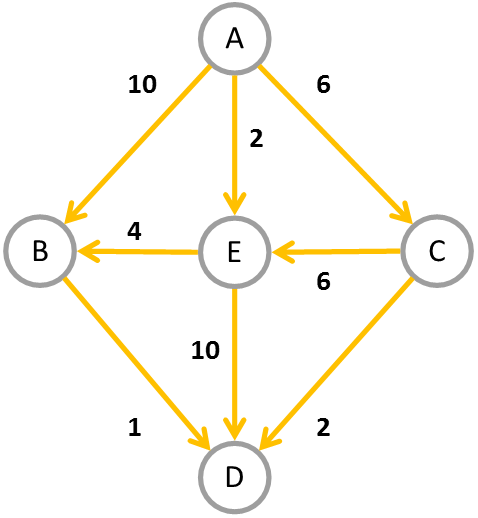
\includegraphics[width=\linewidth]{graphs/spa-graph}
			\captionsetup{justification=centering}
			\caption{The weighted graph $G$.}
			\label{fig:spa-graph}
		\end{subfigure}
		\begin{subfigure}{.4\linewidth}
			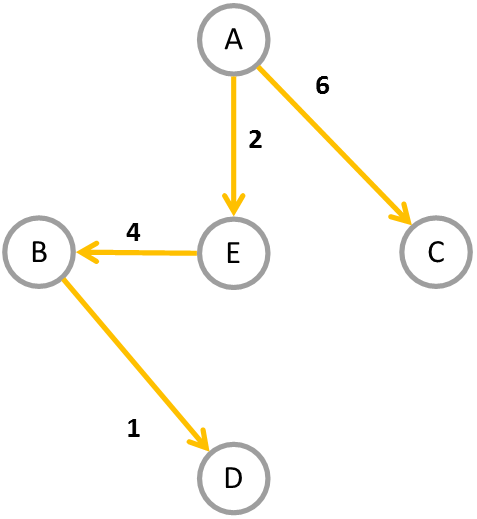
\includegraphics[width=\linewidth]{graphs/spa-tree}
			\captionsetup{justification=centering}
			\caption{The shortest-path tree $S$.}
			\label{fig:spa-tree}
		\end{subfigure}
	\end{figure}
\end{example}

\subsubsection{All-pairs Shortest-path Problem}

Similarly from the previous problem, all-pairs shortest-path is also a search problem that aims to find the predecessors of each vertex $v_i \in V$. The difference is that there is no constraint regarding the initial vertex, i.e., one is interested in finding the shortest routes from every vertex to every other vertex in the graph.

Clearly, all-pairs shortest-path can be solved by executing the Dijkstra's Algorithm $|V|$ times, using every $v_i \in V$ as initial vertex.

\paragraph{Floyd-Warshall Algorithm \cite{golin2003floydwarshall}}

Another solution for the all-pairs shortest-path problem is Floyd-Warshall algorithm, which is entirely based on dynamic programming:

\begin{lstlisting}[mathescape]
    $Floyd-Warshall(w, n)$:
        for $i \in V$
            for $j  \in [1, n]$
                $d(i, j) = w(i, j)$
                $predecessor(i, j) \leftarrow None$

        for $k  \in [1, n]$
            for $j \in [1, n]$
                for $i \in [1, n]$
                    if $d(i, j) > d(i, k) + d(k, j)$
                        $d(i, j) \leftarrow d(i, k) + d(k, j)$
                        $predecessor(i, j) \leftarrow k$
\end{lstlisting}

Now, matrix $d$ contains  the weights sum for the paths between all vertices of the graph. These paths can be constructed by:
\begin{lstlisting}[mathescape]
    $Path(i, j)$:
        if $predecessor(i, j) = None$
            return $[i, j]$
        return $Path(i, pred[i, j]) \bigcup Path(pred[i, j], j)$
\end{lstlisting}

\section{Machine Learning}
“Learning is the improvement of performance is some environment through the acquisition of knowledge resulting from experience in that environment." \cite{pat1996}

According to \cite{hot2009}, “Machine learning is the area in Computer Science that has as goal the projection and implementation of machines that have the ability to learn autonomously”. In other words, the creation of machines that are able to recognize patterns in an environment and interpret those using concepts related to artificial intelligence. Such interpretation can create a model which might eventually be used to predict new patterns, take actions and/or solve domain problems.

\subsection{Machine Learning Algorithms}

Based on how the learning phase of a problem is, most of the ML algorithms may be divided into one of the following categories:

\begin{description}
	\item[Supervised] A direct feedback is presented during the learning phase \cite{pat1996}. For the instances where the ME problem relies on a data set, the learning task uses the labeled training samples (i.e., samples that present the \textbf{target feature}) to synthesize the model that attempts to generalize the relationship between the feature vectors and the target variable \cite{awa2015}.

	\item[Unsupervised] Infer hidden structures from the data set without direct feedback, such as known labels for the samples \cite{awa2015}.

	\item[Semi-supervised] Most commonly, it is given by the extension of either supervised or unsupervised learning to include the other paradigm, resulting in a combination of both \cite{zhu2009}.

	\item[Reinforcement] Through iterative exploration, the learner is positively or negatively reinforced for its actions. The learner's goal is, ultimately, maximize the cumulative reward gained \cite{awa2015}.
\end{description}

\subsection{Support Vector Machine: An Example of Supervised Learning}

The Support Vector Machine algorithm (SVM) is a is a powerful tool, often used in classification problems. Intuitively, the SVM algorithm attempts to find a hyperplane that separates the samples in a data set into two different groups: positives and negatives. Furthermore, the hyperplane is placed such that the distance between the \textbf{support vectors} (the closest samples) and it are maximized.

\begin{figure}[H]
	\centering
	\captionsetup{justification=centering}

	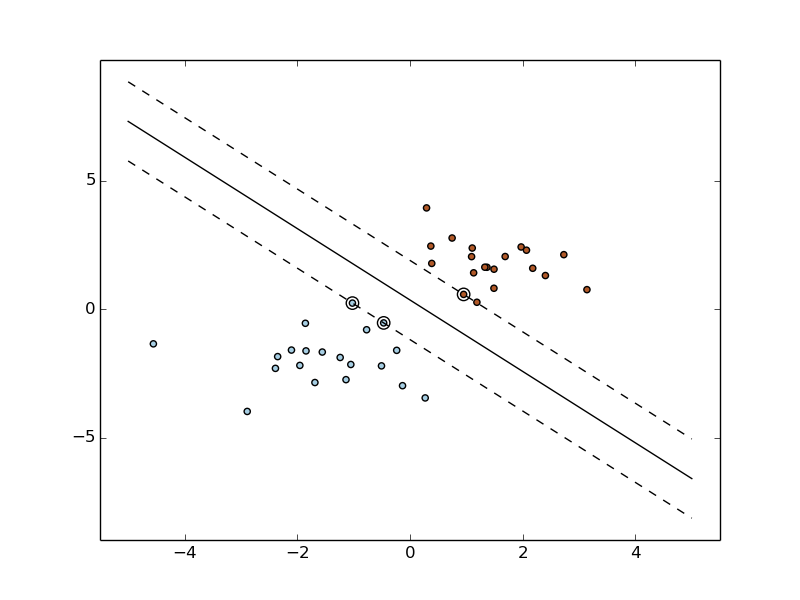
\includegraphics[scale=.5]{svm_margin}
	\caption{A SVM classifier projecting a hyperplane that perfectly separates two classes of samples \cite{sksvm}}.
	\label{fig:svmmargin}
\end{figure}

More elaborately, given any linearly separable data set $X$ containing samples from two distinguished classes $\{-1, +1\}$, consider the vector $w$ a hyperplane $d = \{x \mid w \cdot x + b = 0\}$ (represented in fig. \ref{fig:svmmargin} by the contiguous line) s.t.
$$\text{\textbf{decision rule}} \begin{cases}
	w \cdot u +b \geq 0 \implies y_u=+1\\
	w \cdot u +b < 0 \implies y_u=-1\\
\end{cases}$$

To prevent samples from falling into the margin or being misclassified \cite{wessvmdef}, reinforce that for any positive sample $x_+$, $w \cdot x_+ +b \geq 1$. Similarly for $x_-$ samples, $w \cdot x_- +b \leq 1$. These both constraints can be expressed as
\begin{equation} \label{svmconst}
y_i(w \cdot x_i +b) -1 \geq 0
\end{equation}

Notice that $y_i(w \cdot x_i +b) -1 = 0 \iff x_i $ is a \textbf{support vector}.

The width (the distance between the two margins) of the street is the vector $(x_+^0 -x_-^0)$ projected onto the vector $w$, where $x_-^0$ is a positive support vector and $x_+^0$ is a negative one.
\begin{equation} \label{eq:eqsvmwidth}
\begin{split}
width &= (x_+^0 - x_-^0) \cdot \frac{w}{\|w\|} \\
      &=\frac{x_+^0 \cdot w - x_-^0 \cdot w}{\|w\|} \\
      &=\frac{1-b - (-1-b)}{\|w\|} = \frac{2}{\|w\|}
\end{split}
\end{equation}

As the goal is to maximize the width, while still respecting the constraint (\ref{svmconst}).
\begin{equation} \label{eq:svmminw}
	\max width = \max \frac{2}{\|w\|} \equiv \min \frac{1}{2} \|w\|^2
\end{equation}

Which can be solved using standard quadratic programming.

\subsubsection{SVM for non-separable data sets (soft margins)}

To deal with non-separable data sets, it is possible to introduce the variables $\xi_i$ \cite{wessvmdef}, which represent a trade-off between maximum margin/distance of the misclassified samples from the decision boundary.
$$\min \frac{1}{2} \|w\|^2 + C \sum_{1}^{m}\xi_i \text{, constrained to:}$$
$$y_i(w \cdot x_i +b) \geq 1- \xi_i, \xi_i \geq 0$$

Such trade-off can be adjusted through the parameter $C$. Notice that small values for $C$ might result in misclassification, whereas high values can produce overfitting.

\subsubsection{Dependency over the dot product}

Equation \ref{eq:svmminw} does not explicitly illustrates how the model generated depents on the dot product between the training samples. The implications of such fact will be discussed in the next section. For now, let us convert \ref{eq:svmminw} to its dual form. By the Lagrange multipliers method \cite{mitsvm}:
\begin{align} \label{eq:svmlag1}
	L &= \frac{1}{2}\|w\|^2 - \sum \alpha_i[y_i(w \cdot x_i +b) -1] \\
	\label{svmlag2}
	\frac{\partial L}{\partial w} &= w -\sum\alpha_i y_i x_i = 0 \implies w = \sum\alpha_i y_i x_i \\
	\label{svmlag3}
	\frac{\partial L}{\partial b} &= -\sum\alpha_i y_i = 0 \implies \sum\alpha_i y_i = 0
\end{align}

Applying (\ref{svmlag2}) and (\ref{svmlag3}) on (\ref{eq:svmlag1}), our problem of minimizing (\ref{eq:svmminw}) constrained by (\ref{svmconst}) becomes maximizing $L$, subject to (\ref{svmlag3}):
\begin{gather*}
L = \frac{1}{2}\sum\alpha_i y_i x_i \cdot \sum\alpha_j y_j x_j
- \sum \alpha_i y_i x_i \cdot \sum \alpha_j y_j x_j
- \sum \alpha_i y_i b + \sum \alpha_i \\
= \sum\alpha_i -\frac{1}{2}\sum\sum\alpha_i\alpha_j y_i y_j (x_i \cdot x_j)
\end{gather*}

$w$ and $b$ can easily be found from (\ref{svmlag2}) and $\alpha_i[y_i(w \cdot x_i + b) - 1] = 0$ (for any $i \mid \alpha_i \ne 0$), respectively.

Now, as we finally plug (\ref{svmlag2}) back into our decision rule, it becomes clear that both training and prediction phases depend only on the dot product between the sample vectors \cite{mitsvm}:

$$\text{\textbf{decision rule}} \begin{cases}
	\sum\alpha_i y_i x_i \cdot u +b \geq 0 \implies y_u=+1\\
	\sum\alpha_i y_i x_i \cdot u +b < 0 \implies y_u=-1\\
\end{cases}$$

\subsubsection{Kernel functions}

"The kernel function represent the dot product of both vectors projected onto the new space". \cite{mitsvm}

Some data sets are not linearly separable, as previously mentioned	. They can, however, be projected to a different vector space, where they hopefully will be. To achieve this, a transformation $\phi$ is applied on both vectors. The dot product between those is then calculated in the new space and the value is used during training and prediction:
\begin{gather*}
L = \sum\alpha_i -\frac{1}{2}\sum\sum\alpha_i\alpha_j y_i y_j \phi(x_i) \cdot \phi(x_j)
\end{gather*}

\begin{remark}
	Practically, Let $k: (\mathbb{R}^n, \mathbb{R}^n) \rightarrow \mathbb{R} \mid k(u, v) = \phi(u) \cdot \phi(v)$,
	\begin{gather*}
	L = \sum\alpha_i -\frac{1}{2}\sum\sum\alpha_i\alpha_j y_i y_j k(x_i, x_j)
	\end{gather*}

	Which entails, given a known function $k$, there is no need to explicitly know which are the projections of $x_i$ and $x_j$ onto the new vector space. This is commonly known as the \textbf{kernel trick}.
\end{remark}

$$\text{\textbf{decision rule}} \begin{cases}
\sum\alpha_i y_i k(x_i, u) +b \geq 0 \implies y_u=+1\\
\sum\alpha_i y_i k(x_i, u) +b < 0 \implies y_u=-1\\
\end{cases}$$

The figure bellow illustrates a non-linearly separable data set defined in the $\mathbb{R}$ being projected to the $\mathbb{R}^2$.

\begin{figure}[H]
	\centering
	\captionsetup{justification=centering}

	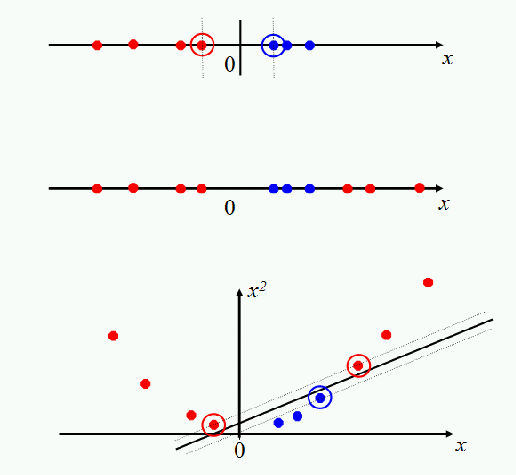
\includegraphics[scale=.4]{svm_kernel}
	\caption{Projection of samples from the $\mathbb{R}$ to the $\mathbb{R}^2$, allowing SVM to find a hyperplane that perfectly separates both classes \cite{svmkernels}.}
	\label{fig:svmkernel}
\end{figure}

Between many different kernels, two often used are the RBF: $\exp(-\frac{\|x -x'\|^2}{2\sigma^2})$ and the Polynomial: $(u^T v + c)^{d}$ \cite{svmkernels}.

\subsection{Multi-class Classification}

Not all problems are binary. In classification, this reflects data sets that have their samples separated into more than two classes. The Iris flower data set is an example of this, when predicting the samples' {\em species}.

There are many different approaches for multi-class classification \cite{rif2008}. For the scope of this work, consider only the following:

\begin{description}
	\item[One-vs-All (OVA)] $n$ binary classifiers are built, where $n$ is also the number of classes in the data set. For the classifier $c^j, j \in [1, n]$, all samples of the $j$th class are taken as positive examples, at the same time that all the other samples are considered negative.

	If
	$$c^j(x) = \sum_{i=1}^{m} y_i \alpha_i^j x \cdot x_i + b$$

	Then positive values for $c^j(x)$ indicate that the sample $x$ belongs to the $j$th class. Additionally, greater $c^j(x)$ values imply on further distance from the hyperplane (i.e., $c^j(x)$ can also be interpreted as a \textbf{confidence value}) and the sample $x$ should be assigned to the class which holds greatest confidence \cite{ovacj}. Shortly, classification is given by
	$$ f(x) = \argmax_j{c^j(x)} $$
	\item[All-vs-All (AVA)] Also known as all-pairs or one-vs-one, a classifier $c_{ij}$ is built for each pair of classes $(i, j)$, resulting in a total of $n(n-1)$ classifiers. $c_{ij}$ responds with positive values for samples of the $i$th class and negative values for samples of the $j$th class. Classification can be done by simply counting the class most frequently associated with $x$:
	$$ f(x) = \argmax_i{\sum_{j=1}^{n} c_{ij}(x)} $$
	Or equivalently, but only using $\frac{n(n-1)}{2}$ classifiers,
	$$ f(x) = \argmax_i{\sum_{j=1}^{n} \frac{j-i}{|j-i|} c_{\min(i, j) \max(i, j)}(x)} $$
\end{description}

\subsection{Evaluating learners}

Machine Learning algorithms might be susceptible to data noise, incorrect configuration or even random factors, which would eventually decrease the generated model's accuracy. In order to evaluate this same accuracy, models are quite often tested after trained.

Considering that testing with the same data used for training will most likely produce unreliable results, a simple way to test a learner is to separate the labeled data set into two chunks, where the first is used for training. The second chunk is then be given to the learner, which attempts to predict the samples. Finally, the predictions made by the learner would be compared with the actual labels.

\subsubsection{Confusion Matrix}

When testing classification models, one way to visualize the wrong predictions made by the learner is a confusion matrix, where the item $a_{ij}$ is the number of times that a sample of the class $i$ was classified as being of the class $j$.

\begin{table}[H]
	\centering
	\begin{tabular}{ |c || *{4}{c|} }
		\hline
           &   a &   b &   c &   d \\\hline\hline
		a & 12 &   3 &   2 &   0 \\
		b &   7 & 12 &   2 &   4 \\
		c &   0 &   4 & 54 &   8 \\
		d &   6 &   0 &   1 & 23 \\\hline
	\end{tabular}

	\caption{Example of confusion matrix for a data-set with four different classes.}
\end{table}

Naturally, a diagonal matrix represents that all samples of the class $i$ were classified as $i$, which is the best possible outcome (no errors).

\subsubsection{Cross Validation}

Sometimes (for example, when the data set does not have too many samples), partitioning of the data set into subsets might be benign to the learning process, as the model will be constructed only considering a small, random portion of the samples. This event is known as \textbf{underfitting}.

When $k$-fold cross-validating \cite{crossvalid}, the data set can be partitioned into $k$ folds. For each fold $k_i$, a model is trained with all folds, except for $k_i$. The model is then tested over $k_i$. Finally, the score reported by the cross-validation method is the average accuracy when testing over all folds.

\subsubsection{Grid Search}

Machine Learning algorithms may require specific parameters to run. For instance, SVM requires $C$ and which $kernel$ it should use. Additionally, kernels might require their own parameters. As these parameters strongly affect how the generated model will be, one cannot choose them arbitrarily.

Grid Search is a traditional method used to find the parameters that optimize the generalization of learning model over a specific data set \cite{gridsearch}. Given a set of possible parameters, it will exhaustively search for the combination of those that generate the best outcome, which might be evaluated by a validation method such as cross-validation.

\subsection{Examples of Learning}

\subsubsection{Coffee Selling Rate}

The figure bellow illustrates the distribution of coffee sales per time of the day in a particular coffee-shop \cite{roh2015}. Clearly being a regression problem, a machine learning algorithm must create a model that appropriately generalizes the distribution observed. Such model will eventually be used to predict the selling rate in the following days.

\begin{figure}[H]
	\centering
	\captionsetup{justification=centering}

	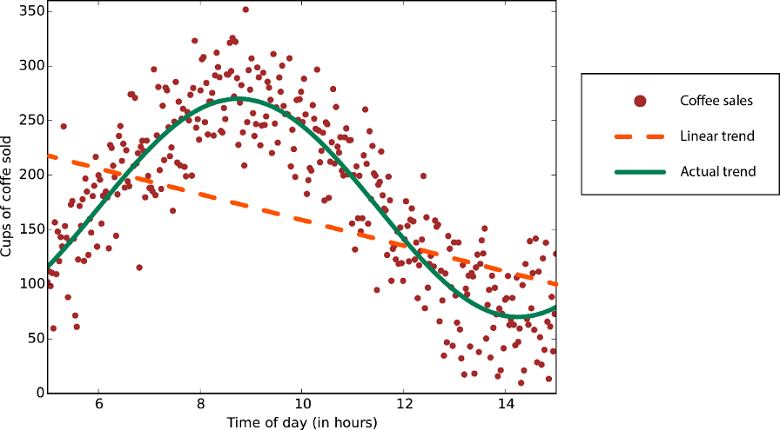
\includegraphics[scale=.4]{rohrer2015}
	\caption{graphic representation of a data set generalization by a linear (orange) and a nonlinear model (green) \cite{roh2015}.}
	\label{fig:rohrer2015}
\end{figure}

The orange line and the green arc represent two different models. The orange line, which represents the linear model, clearly does not generalize the data set appropriately, once it induces an error much larger than necessary \cite{roh2015}. The nonlinear model, i.e., the green arc, was capable of generalize the data inducing a smaller error.

\subsubsection{Iris Flower}

Consider the Iris flower data set as defined in \ref{irisdataset}. In order to predict the feature {\em Species} of a given sample, one could train a Support Vector Machine classifier.

Through GridSearch, it was found that the SVM algorithm with $C=100$, $gamma=.01$ and $rbf$ kernel is capable of finding a model yielding .99\% accuracy. The samples misclassified during the test phase were represented by the confusion matrix bellow.

\begin{figure}[H]
	\centering
	\captionsetup{justification=centering}

	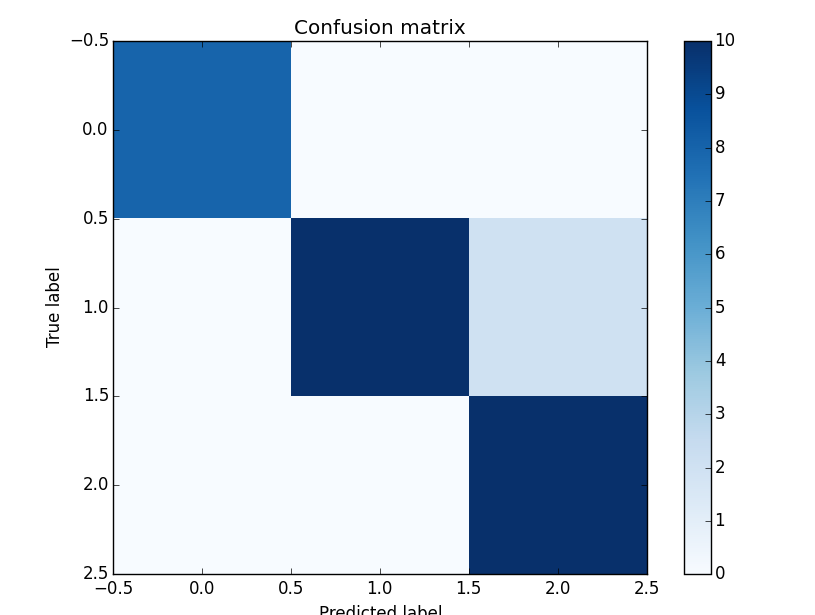
\includegraphics[scale=.2]{svm_cm_iris}
	\caption{Confusion matrix of a SVM with $C=100$, $gamma=.01$ and $rbf$ kernel when predicting samples from the Iris flower data set.}
	\label{fig:cmsvmiris}
\end{figure}
